% ====== Preamble requirements (add once) ======
\usepackage{tikz}
\usetikzlibrary{arrows.meta,positioning,shapes.geometric,calc,fit}
\usepackage{pgfplots}
\pgfplotsset{compat=1.18}

% ==========================================================
% Figure 1: Donor-day selection + day-substitution workflow
% ==========================================================
\begin{figure}[h]
\centering
\begin{tikzpicture}[
  font=\small,
  node distance=7mm and 12mm,
  box/.style={draw, rounded corners, align=center, minimum width=4.4cm, minimum height=8mm},
  decision/.style={draw, diamond, aspect=2, align=center, inner sep=1.5pt, minimum width=3.7cm, minimum height=9mm},
  step/.style={draw, rounded corners, align=left, inner sep=3pt, minimum width=6.6cm},
  dashedstep/.style={draw, dashed, rounded corners, align=left, inner sep=3pt, minimum width=6.6cm},
  arrow/.style={-Latex, thick}
]

% --- Left: gap decomposition per day ---
\node[box] (gap) {Input: gap interval\\(start ts, end ts)};
\node[box, below=of gap] (split) {Split into calendar days\\(D1..Dk) + slot ranges};
\node[box, below=of split] (ctx) {Compute context per missing day\\day\_type, month, dow\\(+ planned exogenous regime)};
\node[box, below=of ctx] (needfull) {For each day: need donor segment\\slots [s\_start..s\_end]};

% --- Right: donor-day selection ladder ---
\node[step, right=22mm of split] (cand0) {\textbf{Build candidate donor set}\\
Filter historical days: near-complete (``good days'')\\
Index by (day\_type, month, dow)};
\node[decision, below=of cand0] (candok) {Candidates\\available?};

\node[step, below left=9mm and 0mm of candok] (ladder) {\textbf{Selection ladder (relax progressively)}\\
1) exact: (day\_type, month, dow)\\
2) relax month: (day\_type, dow)\\
3) relax dow: (day\_type, month)\\
4) relax both: (day\_type)\\
5) global fallback: (any day)};
\node[dashedstep, below=of ladder] (rank) {\textbf{Planned ranking within candidates}\\
Rank by exogenous similarity (e.g., temperature regime)\\
Prefer recent donors / higher data quality};

\node[step, below right=9mm and 0mm of candok] (fallback) {\textbf{If no suitable donors}\\
Use typical profile baseline (fallback tiers)\\
Set LOW quality flag + alert if frequent};

% --- Substitution mechanics ---
\node[box, below=18mm of needfull] (extract) {Extract donor segment\\truncate to slots [s\_start..s\_end]};
\node[box, below=of extract] (scale) {Compute scale from edges\\scale = max(r\_before, r\_after)\\clamp to safe range};
\node[box, below=of scale] (replace) {Replace missing points\\filled = scale $\times$ donor\_segment\\(+ optional mild noise)};
\node[decision, below=of replace] (blendq) {Need boundary\\blending?};

\node[box, below left=9mm and 10mm of blendq] (blend) {Blend edges (local)\\linear interp over k slots\\to match observed neighbor(s)};
\node[box, below right=9mm and 10mm of blendq] (noblend) {No blend\\(pure substitution)};

\node[box, below=18mm of blendq] (meta) {Store metadata\\donor id, match level, scale/clamp\\method + quality flag};

% --- Arrows left track ---
\draw[arrow] (gap) -- (split);
\draw[arrow] (split) -- (ctx);
\draw[arrow] (ctx) -- (needfull);

% --- Arrows to donor selection ---
\draw[arrow] (ctx.east) -- ++(10mm,0) |- (cand0.west);
\draw[arrow] (cand0) -- (candok);

\draw[arrow] (candok) -- node[midway, left, font=\footnotesize] {yes} (ladder);
\draw[arrow] (candok) -- node[midway, right, font=\footnotesize] {no} (fallback);

\draw[arrow] (ladder) -- (rank);
\draw[arrow] (ladder.east) -- ++(8mm,0) |- (extract.east);
\draw[arrow] (rank.east) -- ++(8mm,0) |- (extract.east);
\draw[arrow] (fallback.west) -- ++(-8mm,0) |- (extract.east);

% --- Arrows substitution ---
\draw[arrow] (needfull) -- (extract);
\draw[arrow] (extract) -- (scale);
\draw[arrow] (scale) -- (replace);
\draw[arrow] (replace) -- (blendq);
\draw[arrow] (blendq) -- node[midway, left, font=\footnotesize] {yes} (blend);
\draw[arrow] (blendq) -- node[midway, right, font=\footnotesize] {no} (noblend);

\draw[arrow] (blend) |- (meta);
\draw[arrow] (noblend) |- (meta);

% --- Legend ---
\node[draw, rounded corners, align=left, inner sep=3pt, font=\footnotesize,
      below=10mm of meta, minimum width=12.5cm] (leg) {
\textbf{Legend:} \\
\textit{Truncation} = copy only the donor slots overlapping the missing interval.\\
\textit{Replacement} = insert (scaled) donor values into missing timestamps.\\
\textit{Blending} = local interpolation near boundaries to avoid discontinuities.\\
Dashed box = planned integration (exogenous similarity ranking).
};

\end{tikzpicture}
\caption{Day-substitution logic: donor day selection, truncation to missing slots, replacement, and optional boundary interpolation.}
\end{figure}


% ==========================================================
% Figure 2: Small illustrative plot (partial-day gap filled by donor)
% ==========================================================
\begin{figure}[h]
\centering
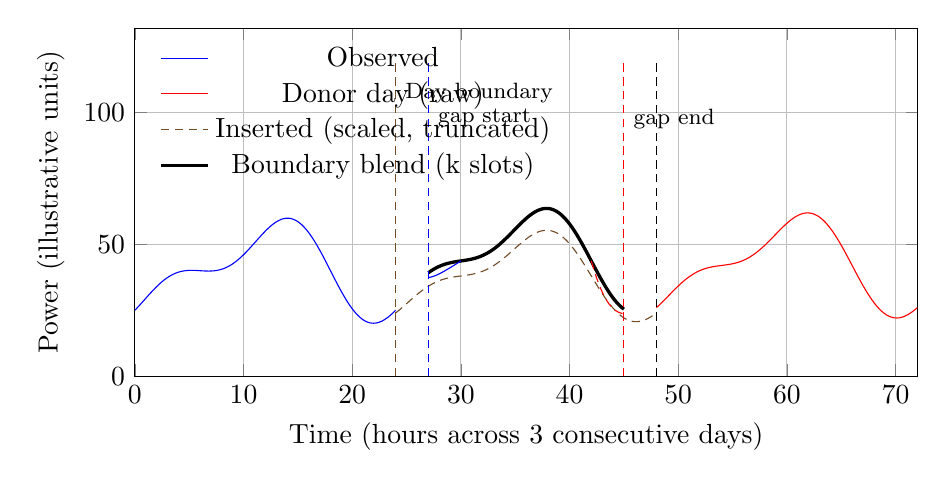
\begin{tikzpicture}
\begin{axis}[
  width=0.95\linewidth,
  height=6.0cm,
  xlabel={Time (hours across 3 consecutive days)},
  ylabel={Power (illustrative units)},
  xmin=0, xmax=72,
  ymin=0,
  legend style={at={(0.02,0.98)},anchor=north west,draw=none,fill=none},
  ymajorgrids=true,
  xmajorgrids=true
]

% --- Observed (Day -1, Day +1) ---
% Day -1: 0..24 (observed)
\addplot+[mark=none] expression[
  domain=0:24,
  samples=200
]{40 + 15*sin(deg(2*pi*(x-6)/24)) + 8*sin(deg(2*pi*(x)/12))};

% Day +1: 48..72 (observed)
\addplot+[mark=none] expression[
  domain=48:72,
  samples=200
]{42 + 16*sin(deg(2*pi*(x-6)/24)) + 7*sin(deg(2*pi*(x)/12))};

\addlegendentry{Observed}

% --- Donor day raw shape (for the missing day, 24..48) ---
\addplot+[mark=none, densely dashed] expression[
  domain=24:48,
  samples=200
]{38 + 14*sin(deg(2*pi*(x-6)/24)) + 6*sin(deg(2*pi*(x)/12))};
\addlegendentry{Donor day (raw)}

% --- Inserted donor segment with scaling (example scale=1.15) ---
% Also shows truncation: only fill 27..45 (partial-day gap),
% leaving 24..27 and 45..48 as "observed" in a real case.
\addplot+[mark=none, very thick] expression[
  domain=27:45,
  samples=200
]{1.15*(38 + 14*sin(deg(2*pi*(x-6)/24)) + 6*sin(deg(2*pi*(x)/12)))};
\addlegendentry{Inserted (scaled, truncated)}

% --- Boundary blending zones (linear interpolation bands, illustrative) ---
% Blend-in: 27..30
\addplot+[mark=none] expression[
  domain=27:30,
  samples=80
]{ ( (30-x)/(30-27) )*(40 + 15*sin(deg(2*pi*(27-6)/24)) + 8*sin(deg(2*pi*(27)/12)))
 + ( (x-27)/(30-27) )*(1.15*(38 + 14*sin(deg(2*pi*(x-6)/24)) + 6*sin(deg(2*pi*(x)/12)))) };
\addlegendentry{Boundary blend (k slots)}

% Blend-out: 42..45
\addplot+[mark=none] expression[
  domain=42:45,
  samples=80
]{ ( (45-x)/(45-42) )*(1.15*(38 + 14*sin(deg(2*pi*(x-6)/24)) + 6*sin(deg(2*pi*(x)/12))))
 + ( (x-42)/(45-42) )*(42 + 16*sin(deg(2*pi*(45-6)/24)) + 7*sin(deg(2*pi*(45)/12))) };

% --- Visual guides: day boundaries and missing interval ---
\addplot+[mark=none] coordinates {(24,0) (24,120)};
\addplot+[mark=none] coordinates {(48,0) (48,120)};
\addplot+[mark=none] coordinates {(27,0) (27,120)};
\addplot+[mark=none] coordinates {(45,0) (45,120)};

\node[anchor=north west] at (axis cs:24,115) {\footnotesize Day boundary};
\node[anchor=north west] at (axis cs:27,105) {\footnotesize gap start};
\node[anchor=north west] at (axis cs:45,105) {\footnotesize gap end};

\end{axis}
\end{tikzpicture}
\caption{Illustrative example of partial-day substitution: a donor day provides the intraday shape, truncated to the missing slot range, scaled using edge ratios, and blended locally near boundaries.}
\end{figure}
